% Options for packages loaded elsewhere
% Options for packages loaded elsewhere
\PassOptionsToPackage{unicode}{hyperref}
\PassOptionsToPackage{hyphens}{url}
%
\documentclass[
  12pt,
]{scrbook}
\usepackage{xcolor}
\usepackage{amsmath,amssymb}
\setcounter{secnumdepth}{5}
\usepackage{iftex}
\ifPDFTeX
  \usepackage[T1]{fontenc}
  \usepackage[utf8]{inputenc}
  \usepackage{textcomp} % provide euro and other symbols
\else % if luatex or xetex
  \usepackage{unicode-math} % this also loads fontspec
  \defaultfontfeatures{Scale=MatchLowercase}
  \defaultfontfeatures[\rmfamily]{Ligatures=TeX,Scale=1}
\fi
\usepackage{lmodern}
\ifPDFTeX\else
  % xetex/luatex font selection
\fi
% Use upquote if available, for straight quotes in verbatim environments
\IfFileExists{upquote.sty}{\usepackage{upquote}}{}
\IfFileExists{microtype.sty}{% use microtype if available
  \usepackage[]{microtype}
  \UseMicrotypeSet[protrusion]{basicmath} % disable protrusion for tt fonts
}{}
\makeatletter
\@ifundefined{KOMAClassName}{% if non-KOMA class
  \IfFileExists{parskip.sty}{%
    \usepackage{parskip}
  }{% else
    \setlength{\parindent}{0pt}
    \setlength{\parskip}{6pt plus 2pt minus 1pt}}
}{% if KOMA class
  \KOMAoptions{parskip=half}}
\makeatother
% Make \paragraph and \subparagraph free-standing
\makeatletter
\ifx\paragraph\undefined\else
  \let\oldparagraph\paragraph
  \renewcommand{\paragraph}{
    \@ifstar
      \xxxParagraphStar
      \xxxParagraphNoStar
  }
  \newcommand{\xxxParagraphStar}[1]{\oldparagraph*{#1}\mbox{}}
  \newcommand{\xxxParagraphNoStar}[1]{\oldparagraph{#1}\mbox{}}
\fi
\ifx\subparagraph\undefined\else
  \let\oldsubparagraph\subparagraph
  \renewcommand{\subparagraph}{
    \@ifstar
      \xxxSubParagraphStar
      \xxxSubParagraphNoStar
  }
  \newcommand{\xxxSubParagraphStar}[1]{\oldsubparagraph*{#1}\mbox{}}
  \newcommand{\xxxSubParagraphNoStar}[1]{\oldsubparagraph{#1}\mbox{}}
\fi
\makeatother


\usepackage{longtable,booktabs,array}
\usepackage{calc} % for calculating minipage widths
% Correct order of tables after \paragraph or \subparagraph
\usepackage{etoolbox}
\makeatletter
\patchcmd\longtable{\par}{\if@noskipsec\mbox{}\fi\par}{}{}
\makeatother
% Allow footnotes in longtable head/foot
\IfFileExists{footnotehyper.sty}{\usepackage{footnotehyper}}{\usepackage{footnote}}
\makesavenoteenv{longtable}
\usepackage{graphicx}
\makeatletter
\newsavebox\pandoc@box
\newcommand*\pandocbounded[1]{% scales image to fit in text height/width
  \sbox\pandoc@box{#1}%
  \Gscale@div\@tempa{\textheight}{\dimexpr\ht\pandoc@box+\dp\pandoc@box\relax}%
  \Gscale@div\@tempb{\linewidth}{\wd\pandoc@box}%
  \ifdim\@tempb\p@<\@tempa\p@\let\@tempa\@tempb\fi% select the smaller of both
  \ifdim\@tempa\p@<\p@\scalebox{\@tempa}{\usebox\pandoc@box}%
  \else\usebox{\pandoc@box}%
  \fi%
}
% Set default figure placement to htbp
\def\fps@figure{htbp}
\makeatother





\setlength{\emergencystretch}{3em} % prevent overfull lines

\providecommand{\tightlist}{%
  \setlength{\itemsep}{0pt}\setlength{\parskip}{0pt}}



 


\usepackage{xcolor}
% define colors
\newcommand{\red}[1]{\color[RGB]{185,64,71}{#1}}
\newcommand{\green}[1]{\color[RGB]{0, 139, 69}{#1}}
\definecolor{red}{RGB}{185,64,71}

% Configure hyperref for expanded bookmarks
% Note that this only works for Adobe Acrobat Reader
\usepackage{hyperref}
\hypersetup{
  bookmarksopen = true, % show TOC with all the subtrees expanded
  bookmarksopenlevel = 2 % level to which bookmarks are open
}

%% bullet list
\usepackage{enumitem}
\setlist[itemize, 1]{
    itemsep = 0.5\baselineskip,
    parsep = 0.2\baselineskip}
\setlist[itemize, 2]{
    itemsep = 0.2\baselineskip
}
\renewcommand{\tightlist}{\setlength{\itemsep}{0.5\baselineskip}\setlength{\parskip}{0.2\baselineskip}}

%% set font
\usepackage{fontspec}
\setmainfont{XCharter}
\setmonofont{Consolas}
\usepackage{unicode-math}
\setmathfont{XCharter-Math.otf} % do NOT delete the .otf extension

%% define custom unicode characters
\usepackage{newunicodechar}
%% for symbols that are not included in the main font, we can use a more symbol robust font to render them, here we use Apple Symbols
\newfontfamily\symbolfont{DejaVu Sans} % Sans is more readable for symbols, rounder and thicker than Serif; Sans Mono is a bit more compact
\newunicodechar{→}{{\symbolfont →}}
\newunicodechar{≈}{{\symbolfont ≈}}
\newunicodechar{⨯}{{\symbolfont ⨯}}
\newunicodechar{♂}{{\symbolfont ♂}}
\newunicodechar{♀}{{\symbolfont ♀}}

%% support for Chinese
\usepackage{xeCJK}
\setCJKmainfont{LXGW WenKai}
\setCJKsansfont{Microsoft YaHei}
\setCJKmonofont{Maple Mono NF CN}

\usepackage{changepage}   % for the adjustwidth environment
\usepackage[all]{nowidow} % prevent widow/orphan lines
\pretolerance = 1000               % Relaxes parameters for line breaks
\tolerance    = 2000               % Relaxes parameters for line breaks


%% table typesetting
\usepackage{threeparttable, adjustbox}
\usepackage{booktabs}
\renewcommand{\arraystretch}{1.3} % increase row spacing
\usepackage{float} % for [H] placement specifier
% Make all tables use [H] placement by default
% Still takes placement, eg [htbp]; defaults to [H] if no placement is specified
\makeatletter
\renewenvironment{table}[1][H]{%
  \@float{table}[#1]%
}{%
  \end@float
}
\makeatother
\usepackage[labelfont={bf}, labelsep=space, skip=4pt]{caption}
\usepackage{siunitx}
% define new column types
\newcommand\mc[1]{\multicolumn{1}{c}{#1}} % center table header
\usepackage{dcolumn}
\newcolumntype{d}[1]{D{.}{.}{#1}} % align at decimal point

%% Math symbols
\usepackage{amsmath, amssymb, textcomp}

%% define TeX macros

% bold face capital letter 大写加粗
\newcommand{\bA}{\boldsymbol{A}}
\newcommand{\bB}{\boldsymbol{B}}
\newcommand{\bC}{\boldsymbol{C}}
\newcommand{\bD}{\boldsymbol{D}}
\newcommand{\bE}{\boldsymbol{E}}
\newcommand{\bF}{\boldsymbol{F}}
\newcommand{\bG}{\boldsymbol{G}}
\newcommand{\bH}{\boldsymbol{H}}
\newcommand{\bI}{\boldsymbol{I}}
\newcommand{\bJ}{\boldsymbol{J}}
\newcommand{\bK}{\boldsymbol{K}}
\newcommand{\bL}{\boldsymbol{L}}
\newcommand{\bM}{\boldsymbol{M}}
\newcommand{\bN}{\boldsymbol{N}}
\newcommand{\bP}{\boldsymbol{P}}
\newcommand{\bQ}{\boldsymbol{Q}}
\newcommand{\bR}{\boldsymbol{R}}
\newcommand{\bS}{\boldsymbol{S}}
\newcommand{\bT}{\boldsymbol{T}}
\newcommand{\bU}{\boldsymbol{U}}
\newcommand{\bV}{\boldsymbol{V}}
\newcommand{\bW}{\boldsymbol{W}}
\newcommand{\bX}{\boldsymbol{X}}
\newcommand{\bY}{\boldsymbol{Y}}
\newcommand{\bZ}{\boldsymbol{Z}}

% bold face small letter 小写加粗
\newcommand{\ba}{\boldsymbol{a}}
\newcommand{\bb}{\boldsymbol{b}}
\newcommand{\bc}{\boldsymbol{c}}
\newcommand{\bd}{\boldsymbol{d}}
\newcommand{\be}{\boldsymbol{e}}
\newcommand{\bg}{\boldsymbol{g}}
\newcommand{\bh}{\boldsymbol{h}}
\newcommand{\bi}{\boldsymbol{i}}
\newcommand{\bm}{\boldsymbol{m}}
\newcommand{\bp}{\boldsymbol{p}}
\newcommand{\bq}{\boldsymbol{q}}
\newcommand{\br}{\boldsymbol{r}}
\newcommand{\bs}{\boldsymbol{s}}
\newcommand{\bt}{\boldsymbol{t}}
\newcommand{\bu}{\boldsymbol{u}}
\newcommand{\bv}{\boldsymbol{v}}
\newcommand{\bw}{\boldsymbol{w}}
\newcommand{\bx}{\boldsymbol{x}}
\newcommand{\by}{\boldsymbol{y}}

% math calligraphic font 花体
\newcommand{\Acal}{\mathcal{A}}
\newcommand{\Bcal}{\mathcal{B}}
\newcommand{\Ccal}{\mathcal{C}}
\newcommand{\Dcal}{\mathcal{D}}
\newcommand{\Ecal}{\mathcal{E}}
\newcommand{\Fcal}{\mathcal{F}}
\newcommand{\Gcal}{\mathcal{G}}
\newcommand{\Hcal}{\mathcal{H}}
\newcommand{\Ical}{\mathcal{I}}
\newcommand{\Jcal}{\mathcal{J}}
\newcommand{\Kcal}{\mathcal{K}}
\newcommand{\Lcal}{\mathcal{L}}
\newcommand{\Mcal}{\mathcal{M}}
\newcommand{\Ncal}{\mathcal{N}}
\newcommand{\Ocal}{\mathcal{O}}
\newcommand{\Pcal}{\mathcal{P}}
\newcommand{\Qcal}{\mathcal{Q}}
\newcommand{\Rcal}{\mathcal{R}}
\newcommand{\Scal}{\mathcal{S}}
\newcommand{\Tcal}{\mathcal{T}}
\newcommand{\Ucal}{\mathcal{U}}
\newcommand{\Vcal}{\mathcal{V}}
\newcommand{\Wcal}{\mathcal{W}}
\newcommand{\Xcal}{\mathcal{X}}
\newcommand{\Ycal}{\mathcal{Y}}
\newcommand{\Zcal}{\mathcal{Z}}

% blackboard face 黑板粗体
\newcommand{\A}{\mathbb{A}}
\newcommand{\B}{\mathbb{B}}
\newcommand{\C}{\mathbb{C}}
\newcommand{\D}{\mathbb{D}}
\newcommand{\E}{\mathbb{E}}
\newcommand{\F}{\mathbb{F}}
\newcommand{\G}{\mathbb{G}}
\renewcommand{\H}{\mathbb{H}}
\newcommand{\I}{\mathbb{I}}
\newcommand{\J}{\mathbb{J}}
\newcommand{\K}{\mathbb{K}}
\renewcommand{\L}{\mathbb{L}}
\newcommand{\M}{\mathbb{M}}
\newcommand{\N}{\mathbb{N}}
\renewcommand{\O}{\mathbb{O}}
\renewcommand{\P}{\mathbb{P}}
\newcommand{\Q}{\mathbb{Q}}
\newcommand{\R}{\mathbb{R}}
\renewcommand{\S}{\mathbb{S}}
\newcommand{\T}{\mathbb{T}}
\newcommand{\U}{\mathbb{U}}
\newcommand{\V}{\mathbb{V}}
\newcommand{\W}{\mathbb{W}}
\newcommand{\X}{\mathbb{X}}
\newcommand{\Y}{\mathbb{Y}}
\newcommand{\Z}{\mathbb{Z}}

% bold face uppercase Greeks
\newcommand{\bAlpha}{\boldsymbol{\Alpha}}
\newcommand{\bBeta}{\boldsymbol{\Beta}}
\newcommand{\bDelta}{\boldsymbol{\Delta}}
\newcommand{\bEta}{\boldsymbol{\eta}}
\newcommand{\bGamma}{\boldsymbol{\Gamma}}
\newcommand{\bLambda}{\boldsymbol{\Lambda}}
\newcommand{\bOmega}{\boldsymbol{\Omega}}
\newcommand{\bPhi}{\boldsymbol{\Phi}}
\newcommand{\bPi}{\boldsymbol{\Pi}}
\newcommand{\bPsi}{\boldsymbol{\Psi}}
\newcommand{\bSigma}{\boldsymbol{\Sigma}}
\newcommand{\bTau}{\boldsymbol{\tau}}
\newcommand{\bXi}{\boldsymbol{\Xi}}

% bold face lowercase Greeks
\newcommand{\bbeta}{\boldsymbol{\beta}}
\newcommand{\bdelta}{\boldsymbol{\delta}}
\newcommand{\blambda}{\boldsymbol{\lambda}}
\newcommand{\bmu}{\boldsymbol{\mu}}
\newcommand{\bphi}{\boldsymbol{\phi}}
\newcommand{\bpi}{\boldsymbol{\pi}}
\newcommand{\bpsi}{\boldsymbol{\psi}}
\newcommand{\brho}{\boldsymbol{\rho}}
\newcommand{\bsigma}{\boldsymbol{\sigma}}
\newcommand{\btau}{\boldsymbol{\tau}}
\newcommand{\bxi}{\boldsymbol{\xi}}

% Functions (single argument)
\newcommand{\curl}[1]{\left\lbrace #1 \right\rbrace}
\newcommand{\floor}[1]{\left\lfloor #1 \right\rfloor}
\newcommand{\ceil}[1]{\left\lceil #1 \right\rceil}
\newcommand{\abs}[1]{\left\lvert #1 \right\rvert}
\newcommand{\norm}[1]{\left\lVert #1 \right\rVert}

% Other operators
\newcommand{\var}{\mathrm{Var}}
\newcommand{\cov}{\mathrm{Cov}}
\newcommand{\cor}{\mathrm{Corr}}
\newcommand{\diag}{\mathrm{diag}}
\newcommand{\rank}{\mathrm{rank}}
\newcommand{\vecc}{\mathrm{vec}}
\newcommand{\indep}{\perp \! \! \! \perp}

% Remove "0." prefix from subsection and subsubsection numbering
\makeatletter
\renewcommand{\thesubsection}{%
  \ifnum\value{section}=0
    \arabic{subsection}%
  \else
    \thesection.\arabic{subsection}%
  \fi
}
\renewcommand{\thesubsubsection}{%
  \ifnum\value{subsection}=0
    \ifnum\value{section}=0
      \arabic{subsubsection}%
    \else
      \thesection.\arabic{subsubsection}%
    \fi
  \else
    \ifnum\value{section}=0
      \arabic{subsection}.\arabic{subsubsection}%
    \else
      \thesection.\arabic{subsection}.\arabic{subsubsection}%
    \fi
  \fi
}
\makeatother
\usepackage{xcolor}
\usepackage{colortbl}
\makeatletter
\@ifpackageloaded{tcolorbox}{}{\usepackage[skins,breakable]{tcolorbox}}
\@ifpackageloaded{fontawesome5}{}{\usepackage{fontawesome5}}
\definecolor{quarto-callout-color}{HTML}{909090}
\definecolor{quarto-callout-note-color}{HTML}{0758E5}
\definecolor{quarto-callout-important-color}{HTML}{CC1914}
\definecolor{quarto-callout-warning-color}{HTML}{EB9113}
\definecolor{quarto-callout-tip-color}{HTML}{00A047}
\definecolor{quarto-callout-caution-color}{HTML}{FC5300}
\definecolor{quarto-callout-color-frame}{HTML}{acacac}
\definecolor{quarto-callout-note-color-frame}{HTML}{4582ec}
\definecolor{quarto-callout-important-color-frame}{HTML}{d9534f}
\definecolor{quarto-callout-warning-color-frame}{HTML}{f0ad4e}
\definecolor{quarto-callout-tip-color-frame}{HTML}{02b875}
\definecolor{quarto-callout-caution-color-frame}{HTML}{fd7e14}
\makeatother
\makeatletter
\@ifpackageloaded{caption}{}{\usepackage{caption}}
\AtBeginDocument{%
\ifdefined\contentsname
  \renewcommand*\contentsname{Table of contents}
\else
  \newcommand\contentsname{Table of contents}
\fi
\ifdefined\listfigurename
  \renewcommand*\listfigurename{List of Figures}
\else
  \newcommand\listfigurename{List of Figures}
\fi
\ifdefined\listtablename
  \renewcommand*\listtablename{List of Tables}
\else
  \newcommand\listtablename{List of Tables}
\fi
\ifdefined\figurename
  \renewcommand*\figurename{Figure}
\else
  \newcommand\figurename{Figure}
\fi
\ifdefined\tablename
  \renewcommand*\tablename{Table}
\else
  \newcommand\tablename{Table}
\fi
}
\@ifpackageloaded{float}{}{\usepackage{float}}
\floatstyle{ruled}
\@ifundefined{c@chapter}{\newfloat{codelisting}{h}{lop}}{\newfloat{codelisting}{h}{lop}[chapter]}
\floatname{codelisting}{Listing}
\newcommand*\listoflistings{\listof{codelisting}{List of Listings}}
\usepackage{amsthm}
\theoremstyle{definition}
\newtheorem{example}{Example}[section]
\theoremstyle{remark}
\AtBeginDocument{\renewcommand*{\proofname}{Proof}}
\newtheorem*{remark}{Remark}
\newtheorem*{solution}{Solution}
\newtheorem{refremark}{Remark}[section]
\newtheorem{refsolution}{Solution}[section]
\makeatother
\makeatletter
\makeatother
\makeatletter
\@ifpackageloaded{caption}{}{\usepackage{caption}}
\@ifpackageloaded{subcaption}{}{\usepackage{subcaption}}
\makeatother
\usepackage{bookmark}
\IfFileExists{xurl.sty}{\usepackage{xurl}}{} % add URL line breaks if available
\urlstyle{same}
\hypersetup{
  pdftitle={Probability and Data in Business Analytics},
  hidelinks,
  pdfcreator={LaTeX via pandoc}}


\title{Probability and Data in Business Analytics}
\author{}
\date{}
\begin{document}
\frontmatter
\maketitle


\mainmatter
\begin{tcolorbox}[enhanced jigsaw, left=2mm, rightrule=.15mm, opacityback=0, arc=.35mm, leftrule=.75mm, colframe=quarto-callout-note-color-frame, bottomrule=.15mm, colback=white, breakable, toprule=.15mm]

🎯 \textbf{Study Objectives}

\begin{itemize}
\tightlist
\item
  Apply probability rules to real business events.
\item
  Distinguish clearly between population parameters and sample
  estimators.
\item
  Compute and explain expectation, variance, and standard deviation in
  business contexts.
\item
  Interpret higher moments: skewness and kurtosis for tail and asymmetry
  assessment.
\item
  Combine random variables (e.g., portfolio or multi‑channel forecast)
  and decompose variance with covariance terms.
\item
  Calculate and interpret covariance and correlation; relate
  independence vs.~zero correlation.
\end{itemize}

\end{tcolorbox}

Probability is the foundation for making data-driven decisions in
business. This section covers the essential concepts, formulas, and
business examples you'll use in analytics.

\section{Probability Axioms}\label{probability-axioms}

Probability measures how likely an event is.

\[P(A) = \frac{\text{Number of ways A can occur}}{\text{Total possible outcomes}}\]

\begin{enumerate}
\def\labelenumi{\arabic{enumi}.}
\tightlist
\item
  \(P(A) \geq 0\) for any event \(A\)
\item
  \(P(\text{all possible outcomes}) = 1\)
\item
  \(P(A \text{ or } B) = P(A) + P(B) - P(A\text{ and }B)\)
\item
  If \(A\) and \(B\) are mutually exclusive, then \[
  P(A \text{ and } B) = 0
  \] and \[
  P(A \text{ or } B) = P(A) + P(B)
  \] Mutually exclusive means ``cannot happen together.''
\end{enumerate}

\begin{example}[]\protect\hypertarget{exm-1}{}\label{exm-1}

A retailer estimates a 30\% chance of a supply chain disruption and a
50\% chance of a demand spike. If these events are mutually exclusive,
what is the probability of either event occurring?

\end{example}

Solution

\begin{refsolution}
Since the events are mutually exclusive, \(P(A \text{ and } B)=0,\) then
\[
\begin{split}
P(A \text{ and } B)=P(A)+P(B)-P(A \text{ and } B)=0.30+0.50=0.80.
\end{split}
\]

\label{sol-1}

\end{refsolution}

\begin{example}[]\protect\hypertarget{exm-2}{}\label{exm-2}

In a multi-channel marketing campaign, 35\% of customers click an email
offer (Event A) and 25\% engage with a social media ad (Event B). Data
shows 10\% of customers do both. What is the probability a randomly
selected customer engages with at least one of the two channels (email
OR social)?

\end{example}

Solution

\begin{refsolution}
\leavevmode

\(P(A) + P(B) - P(A \text{ and } B) = 0.35 + 0.25 - 0.10 = 0.50\)

\label{sol-2}

\end{refsolution}

\section{Sample vs.~Population: Estimating the Big
Picture}\label{sample-vs.-population-estimating-the-big-picture}

In business, we use samples to estimate population characteristics.

Sample mean:

\[
\overline{X} = \frac{1}{n} \sum_{i=1}^n X_i
\]

\begin{example}[]\protect\hypertarget{exm-telecom}{}\label{exm-telecom}

A telecom company surveys a randomly selected sample of 500 customers
about service quality. The sample mean satisfaction score is 4.2. How
can this estimate help guide company-wide improvements?

\end{example}

Solution

\begin{refsolution}
\leavevmode

\begin{itemize}
\tightlist
\item
  The sample mean (4.2) is based on 500 surveyed customers (the sample).
\item
  The population is all customers of the telecom company.
\item
  To guide company-wide improvements, we need to know if the sample is
  representative of the population.
\item
  There is uncertainty in the estimate; larger samples make the sample
  mean closer to the true population mean.
\item
  The sample mean is useful, but its reliability depends on sample
  representativeness and size.
\end{itemize}

\label{sol-telecom}

\end{refsolution}

\begin{example}[]\protect\hypertarget{exm-3}{}\label{exm-3}

Why is it important to distinguish between sample and population in
business analytics?

\end{example}

Solution

\begin{refsolution}
\leavevmode

Because we use samples to estimate population parameters, and
understanding the difference helps us make better decisions and avoid
bias.

\label{sol-3}

\end{refsolution}

\section{Moments}\label{moments}

\subsection{Expectation, Variance, and Standard
Deviation}\label{expectation-variance-and-standard-deviation}

\begin{itemize}
\item
  \textbf{Expectation (population):} Average level of the outcome (true
  but unknown in practice). \[
  \mathbb{E}[X] =
  \begin{cases}
  \displaystyle \sum_{i} x_i \, P(X = x_i) & \text{(discrete)} \\
  \displaystyle \int_{-\infty}^{\infty} x \, f(x) \, dx & \text{(continuous)} \\
  \end{cases}
  \] \textbf{Sample estimator:} Replace the distribution by observed
  data: \[\bar{X} = \dfrac{1}{n}\sum_{i=1}^n X_i.\] The sample mean
  \(\bar{X}\) estimates the population mean \(\mathbb{E}[X]\).
\item
  \textbf{Variance (population):} How much values fluctuate around the
  true mean.

  \[\text{Var}(X) = E[(X - E[X])^2]\]

  The variance can also be expressed as:

  \[
  \begin{aligned}
  \color[HTML]{00CC66}{\text{Var}(X)} &= \mathbb{E}\left[\left(X - \mathbb{E}[X]\right)^2\right] \\
  &= \color[HTML]{00CC66}{\mathbb{E}[X^2] - (\mathbb{E}[X])^2}.
  \end{aligned}
  \]

  This second form is often faster to compute when you already have (or
  can easily get) \(\mathbb{E}[X^2]\) (e.g., from grouped data or a
  probability model). In finance, we frequently estimate variance from
  simulated or historical returns by computing the average of squared
  returns (giving \(\mathbb{E}[X^2]\)) and subtracting the square of the
  average return.

  \textbf{Sample estimators:}

  \begin{itemize}
  \tightlist
  \item
    \textbf{Biased} (population style) estimator:
    \[ \hat{\sigma}^2 = \dfrac{1}{n}\sum_{i=1}^n (X_i - \bar{X})^2 \]
  \item
    \textbf{Unbiased} estimator:
    \[s^2 = \dfrac{1}{n-1}\sum_{i=1}^n (X_i - \bar{X})^2 \] The latter
    (\(s^2\)) subtracts 1 from \(n\) in the denominator, which is known
    as a {degrees of freedom correction}. This version has some
    desirable properties but we will not discuss these for now. Suffice
    to say that both versions are usually fine in practice.
  \end{itemize}
\end{itemize}

\begin{example}[]\protect\hypertarget{exm-10}{}\label{exm-10}

An operations planner models next-hour demand arrivals for a
micro-warehouse (number of urgent orders) as \(X \in \{0,1,2\}\) with
probabilities 0.2, 0.5, 0.3. Compute the variability (variance) of order
arrivals using the shortcut formula
\(\mathbb{E}[X^2] - (\mathbb{E}[X])^2\) to inform staffing.

\end{example}

Solution

\begin{refsolution}
\[
\begin{split}
\mathbb{E}[X] &= 0(0.2)+1(0.5)+2(0.3)=1.1 \\
\mathbb{E}[X^2] &= 0^2(0.2)+1^2(0.5)+2^2(0.3)=0+0.5+1.2=1.7 \\
\text{Var}(X) &= \mathbb{E}[X^2] - (\mathbb{E}[X])^2 = 1.7 - 1.1^2 = 1.7 - 1.21 = 0.49
\end{split}
\]

\label{sol-10}

\end{refsolution}

\begin{example}[]\protect\hypertarget{exm-11}{}\label{exm-11}

A SaaS company tracks daily change in Daily Active Users (DAU) (in \%)
over 5 days: \(0.4\), \(0.6\), \(-0.2\), \(0.5\), \(0.7\). Verify that
the direct variance definition and the shortcut formula match; interpret
what the variance implies for short‑term engagement volatility.

\end{example}

Solution

\begin{refsolution}
Daily \% changes: \(0.4,\ 0.6,\ -0.2,\ 0.5,\ 0.7\). Let units be
\textbf{percentage points} (pp). \[
\mathbb{E}[X] = \frac{0.4+0.6-0.2+0.5+0.7}{5} = 0.4 \text{ pp}
\] \[
\mathbb{E}[X^2] = \frac{0.16+0.36+0.04+0.25+0.49}{5} = \frac{1.30}{5} = 0.26 \text{ (pp)}^2
\] Variance (percentage-point squared): \[
\text{Var}(X) = 0.26 - (0.4)^2 = 0.26 - 0.16 = 0.10 \text{ (pp)}^2
\] Standard deviation \(= \sqrt{0.10} \approx 0.316\) pp (about \(0.32\)
percentage points). Direct (long) method matches (0.10).\\
Interpretation: Moderate short-term volatility compared to the mean
change of 0.4 pp.~This suggests some fluctuations in user engagement,
but not extreme.

\label{sol-11}

\end{refsolution}

\begin{itemize}
\item
  \textbf{Standard Deviation (population):} Square root of variance,
  showing average deviation from the true mean.

  \[\text{sd}(X) = \sqrt{\text{Var}(X)}\]

  \textbf{Sample estimator:} \(s = \sqrt{s^2}\) (using the unbiased
  \(s^2\) above).
\end{itemize}

\begin{example}[]\protect\hypertarget{exm-9}{}\label{exm-9}

A hedge fund analyzes daily returns of two portfolios. Portfolio A has
higher mean but also higher variance. How should risk-adjusted
performance be compared?

\end{example}

Solution

\begin{refsolution}
\leavevmode

Compare risk-adjusted metrics (e.g., Sharpe ratio = (mean - rf)/sd).
Higher mean with disproportionate variance may yield lower Sharpe.

\label{sol-9}

\end{refsolution}

\begin{example}[]\protect\hypertarget{exm-4}{}\label{exm-4}

A business has daily profits of \$200, \$250, \$180, \$220, and \$210.
Calculate the mean and variance.

\end{example}

Solution

\begin{refsolution}
\textbf{Mean:}
\(\bar{x}=\dfrac{200+250+180+220+210}{5}=\dfrac{1060}{5}=212\).

\textbf{Variance calculations:}

\begin{enumerate}
\def\labelenumi{\arabic{enumi}.}
\tightlist
\item
  \textbf{Sum of squared deviations}\\
  \[
  \begin{aligned}
  (200-212)^2 &+ (250-212)^2 + (180-212)^2 + (220-212)^2 + (210-212)^2 \\
  &= 144 + 1444 + 1024 + 64 + 4 = 2680
  \end{aligned}
  \]
\item
  \textbf{Population variance} (divide by \(n=5\))\\
  \[ \sigma^2 = \frac{2680}{5} = 536 \]
\item
  \textbf{Sample variance} (unbiased, divide by \(n-1=4\))\\
  \[ s^2 = \frac{2680}{4} = 670 \]
\end{enumerate}

Population variance uses \(n\) when treating these 5 observations as the
entire population; sample variance uses \(n-1\) to unbiasedly estimate
\(\text{Var}(X)\) of a larger process.

\label{sol-4}

\end{refsolution}

\subsection{Sums of Random Variables: Expectation \&
Variance}\label{sums-of-random-variables-expectation-variance}

Population linearity of expectation: \[E[X + Y] = E[X] + E[Y]\]

Sample counterpart: \(\overline{X+Y} = \bar{X} + \bar{Y}\) (sample means
add componentwise).

If \(X\) and \(Y\) are independent, the population variance of their sum
is the sum of their variances:
\[\text{Var}(X + Y) = \text{Var}(X) + \text{Var}(Y)\]

If not independent, add twice the covariance:
\[\text{Var}(X + Y) = \text{Var}(X) + \text{Var}(Y) + 2\text{Cov}(X, Y)\]

Sample counterpart (unbiased style):
\[s_{X+Y}^2 = s_X^2 + s_Y^2 + 2 s_{XY},\] where
\(s_{XY} = \dfrac{1}{n-1}\sum_{i=1}^n (X_i-\bar{X})(Y_i-\bar{Y}).\)

\textbf{Intuitive Example:} In portfolio management, the total risk
(variance) of a portfolio depends on the variances of individual assets
and how they move together (covariance).

\begin{example}[]\protect\hypertarget{exm-6}{}\label{exm-6}

Two independent projects have profit variances of 100 and 150. What is
the variance of total profit?

\end{example}

Solution

\begin{refsolution}
\leavevmode

\(100 + 150 = 250\).

\label{sol-6}

\end{refsolution}

\subsubsection{Variance of Linear Transformations \&
Portfolios}\label{variance-of-linear-transformations-portfolios}

The variance operator is the expectation of a quadratic function, so it
is not linear. Instead, for constants \(a, b\):

\[
\text{Var}(a + bX) = b^2\,\text{Var}(X).
\]

More generally, for constants \(a_i \in \mathbb{R}, i=1,\ldots,n\):

\[
\text{Var}\left(\sum_{i=1}^n a_i X_i \right) = \sum_{i=1}^n a_i^2 \, \text{Var}(X_i) + \sum_{i=1}^n \sum_{j=1}^n a_i a_j \, \text{Cov}(X_i, X_j).
\]

If the \(X_i\) are pairwise independent (or uncorrelated), the double
sum of covariance terms drops out for \(i\neq j\), leaving only the
first sum.

\begin{example}[]\protect\hypertarget{exm-12}{}\label{exm-12}

A portfolio allocates 40\% to Asset A and 60\% to Asset B.
\(\text{Var}(A)=0.04\), \(\text{Var}(B)=0.09\), and
\(\text{Cov}(A,B)=0.01\). Compute portfolio variance using the general
formula.

\end{example}

Solution

\begin{refsolution}
\leavevmode

\(\text{Var}(P)=0.4^2(0.04)+0.6^2(0.09)+2(0.4)(0.6)(0.01)=0.0064+0.0324+0.0048=0.0436\).

\label{sol-12}

\end{refsolution}

\begin{example}[]\protect\hypertarget{exm-13}{}\label{exm-13}

A production planner combines forecasts: Final forecast
\(F = 2 + 0.7X_1 + 0.3X_2\). If \(\text{Var}(X_1)=25\),
\(\text{Var}(X_2)=9\), and \(\text{Cov}(X_1,X_2)=6\), find
\(\text{Var}(F)\).

\end{example}

Solution

\begin{refsolution}
\leavevmode

Constant 2 adds no variance.
\(\text{Var}(F)=0.7^2(25)+0.3^2(9)+2(0.7)(0.3)(6)=12.25+0.81+2.52=15.58\).

\label{sol-13}

\end{refsolution}

\subsection{Skewness}\label{skewness}

Skewness measures asymmetry in a distribution.

\begin{itemize}
\tightlist
\item
  \textbf{Skewness = 0:} Symmetric (e.g., normal)
\item
  \textbf{Skewness \textless{} 0:} Longer left tail (large losses more
  likely than large gains)
\item
  \textbf{Skewness \textgreater{} 0:} Longer right tail (occasional big
  gains)
\end{itemize}

\begin{figure}[H]

\centering{

\includegraphics[width=0.7\linewidth,height=\textheight,keepaspectratio]{images/Skewness.png}

}

\caption{\label{fig-skew}Diagram of Skewness.}

\end{figure}%

Business reading: Positive skew in quarterly sales means you usually hit
average numbers but sometimes land a very big contract. Negative skew in
operational losses could mean rare but severe downside events that need
contingency planning.

Let \(\mu_3 = E[(X-\mathbb{E}[X])^3]\) denote the third central moment.
Standardized (population) skewness:
\[\gamma_1 = \frac{\mu_3}{\text{sd}(X)^3}.\]

Sample (bias‑adjusted) skewness estimator:
\[\hat{\gamma}_1 = \frac{n}{(n-1)(n-2)} \sum_{i=1}^n \left(\frac{X_i-\bar{X}}{s}\right)^3.\]

\begin{tcolorbox}[enhanced jigsaw, title=\textcolor{quarto-callout-tip-color}{\faLightbulb}\hspace{0.5em}{Tip}, bottomtitle=1mm, bottomrule=.15mm, toprule=.15mm, colbacktitle=quarto-callout-tip-color!10!white, left=2mm, rightrule=.15mm, coltitle=black, opacitybacktitle=0.6, leftrule=.75mm, toptitle=1mm, colframe=quarto-callout-tip-color-frame, titlerule=0mm, colback=white, breakable, arc=.35mm, opacityback=0]

Note for skewness and kurtosis, it is NOT expected to hand calculate the
values, the focus is on

\begin{itemize}
\tightlist
\item
  the interpretation of given results.
\item
  be able to recognize skewness and kurtosis in data visualizations
  (e.g., histograms, box plots).
\end{itemize}

\end{tcolorbox}

\subsection{Kurtosis}\label{kurtosis}

Kurtosis measures tail weight (propensity for outliers) relative to a
normal distribution.

\begin{itemize}
\tightlist
\item
  \textbf{Kurtosis ≈ 3:} Normal tail thickness
\item
  \textbf{Kurtosis \textgreater{} 3 (leptokurtic):} Heavy / fat tails,
  more extreme outcomes
\item
  \textbf{Kurtosis \textless{} 3 (platykurtic):} Light / thin tails,
  fewer extremes
\end{itemize}

\begin{figure}[H]

\centering{

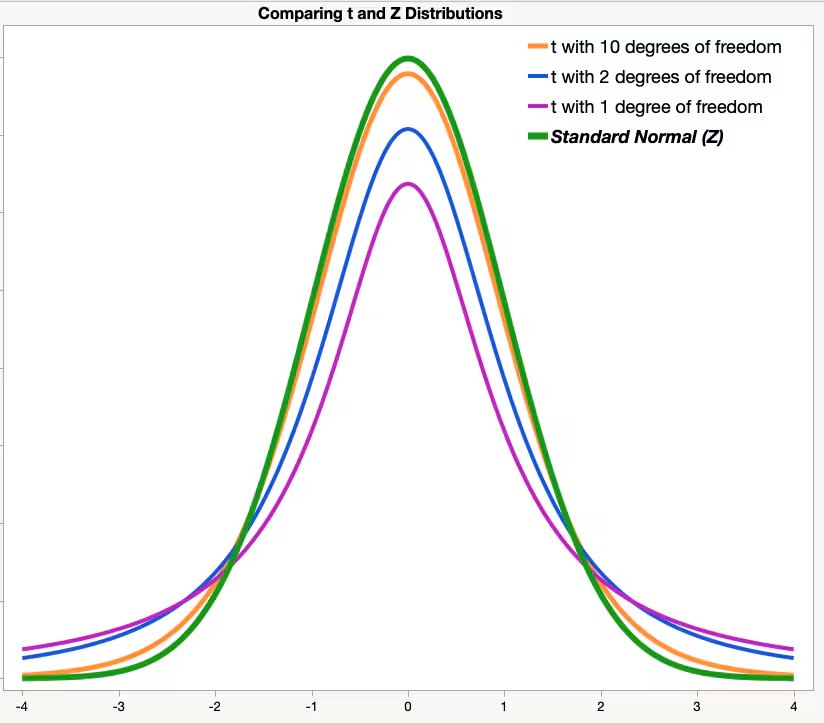
\includegraphics[width=0.7\linewidth,height=\textheight,keepaspectratio]{images/t_distribution2.png}

}

\caption{\label{fig-t}Examples of heavy-tailed distributions.}

\end{figure}%

{\(t\)-distribution} has \emph{higher} kurtosis than normal
distributions.

\begin{itemize}
\tightlist
\item
  Meaning that \(t\)-distribution has a higher probability of obtaining
  values that are far from the mean than a normal distribution.
\item
  It is less peaked in the center and higher in the tails than normal
  distribution.
\item
  As the degree of freedom increases, \(t\)-distribution approximates to
  normal distribution, kurtosis decreases and approximates to 3.
\end{itemize}

\begin{figure}[H]

\centering{

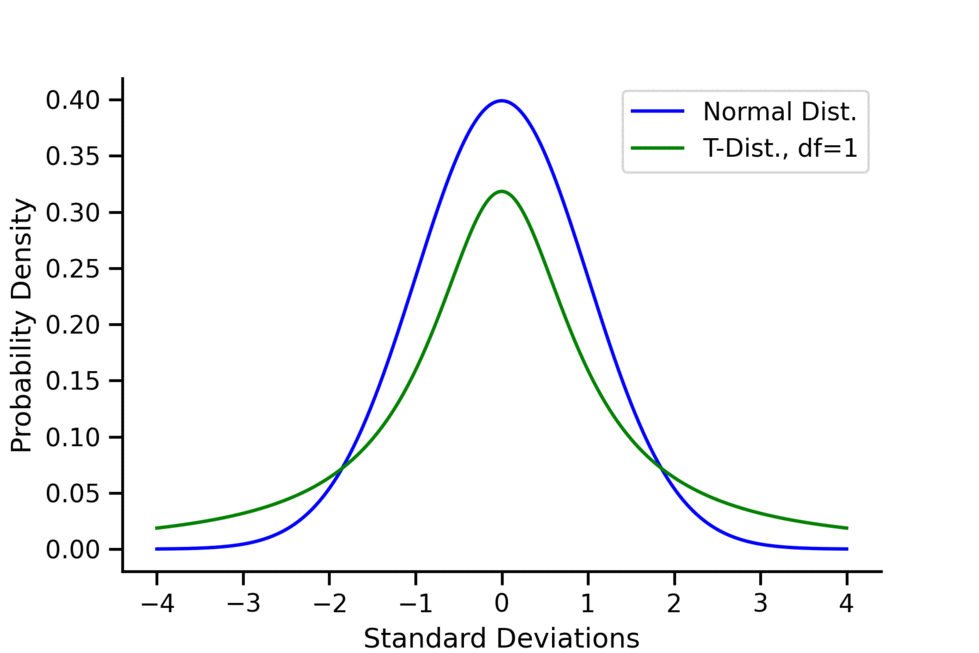
\includegraphics[width=0.8\linewidth,height=\textheight,keepaspectratio]{images/t-dist_chang_df_static.png}

}

\caption{\label{fig-t-dist-change-df}The comparison between the
\emph{t}-distribution and the normal distribution at degrees of freedom
ranging from 1 to 50. Figure source: from
\href{https://tjkyner.medium.com/the-normal-distribution-vs-students-t-distribution-322aa12ffd15}{T.J.
Kyner}.}

\end{figure}%

\begin{tcolorbox}[enhanced jigsaw, title=\textcolor{quarto-callout-tip-color}{\faLightbulb}\hspace{0.5em}{For the \(t\)-distribution:}, bottomtitle=1mm, bottomrule=.15mm, toprule=.15mm, colbacktitle=quarto-callout-tip-color!10!white, left=2mm, rightrule=.15mm, coltitle=black, opacitybacktitle=0.6, leftrule=.75mm, toptitle=1mm, colframe=quarto-callout-tip-color-frame, titlerule=0mm, colback=white, breakable, arc=.35mm, opacityback=0]

\begin{itemize}
\tightlist
\item
  As the degrees of freedom (df) increase, the \(t\)-distribution
  approaches the normal distribution.
\item
  A common rule of thumb is that for \(df > 30\), one can pretty safely
  use the normal distribution in place of a \emph{t}-distribution unless
  you are interested in the extreme tails.
\end{itemize}

\end{tcolorbox}

Let \(\mu_4 = E[(X-\mathbb{E}[X])^4]\) be the fourth central moment.
Standardized (population) kurtosis:
\[\kappa = \frac{\mu_4}{\text{sd}(X)^4}, \qquad \text{Excess kurtosis} = \kappa - 3.\]
Sample (Fisher) excess kurtosis estimator:
\[\hat{g}_2 = \frac{n(n+1)}{(n-1)(n-2)(n-3)} \sum_{i=1}^n \left(\frac{X_i-\bar{X}}{s}\right)^4 - \frac{3(n-1)^2}{(n-2)(n-3)}.\]
High excess kurtosis signals greater tail risk; low or negative excess
indicates fewer extreme outcomes.

Interpretation link: High positive skewness without high kurtosis means
upside spikes with limited extra tail risk; high kurtosis (regardless of
skew sign) means fatter tails and a need to focus on outlier management.

\begin{example}[]\protect\hypertarget{exm-5}{}\label{exm-5}

A company's quarterly profits have excess kurtosis of 4. What does this
mean for risk management?

\end{example}

Solution

\begin{refsolution}
Excess kurtosis is defined relative to a normal distribution (which has
kurtosis 3).

\begin{itemize}
\tightlist
\item
  Excess kurtosis = Kurtosis − 3
\item
  So an excess kurtosis of 4 means the total kurtosis is \textbf{7},
  much higher than a normal distribution.
\end{itemize}

This implies the distribution of quarterly profits has \textbf{fat
tails} --- extreme profit or loss outcomes are more likely than under a
normal distribution. Recommend to focus risk management on outliers.

\label{sol-5}

\end{refsolution}

\section{Covariance, Correlation \&
Independence}\label{covariance-correlation-independence}

Population covariance measures the direction of comovement between two
variables:

\begin{itemize}
\tightlist
\item
  \textbf{Positive covariance:} Both variables increase or decrease
  together
\item
  \textbf{Negative covariance:} One increases while the other decreases
\item
  \textbf{Magnitude:} Does not indicate strength of relationship
\end{itemize}

\textbf{Population formulas:}
\[\text{Cov}(X, Y) = E[(X - E[X])(Y - E[Y])]\]
\[\text{Cov}(X, Y) = E[XY] - E[X]E[Y]\]

\textbf{Sample covariance (unbiased):}
\[s_{XY} = \frac{1}{n-1}\sum_{i=1}^n (X_i - \bar{X})(Y_i - \bar{Y}).\]

Population correlation standardizes covariance to a scale from -1 to 1:
\[\text{Corr}(X, Y) = \frac{\text{Cov}(X, Y)}{\text{sd}(X) \cdot \text{sd}(Y)}\]

\textbf{Sample correlation:} \[r_{XY} = \frac{s_{XY}}{s_X s_Y}.\]

\begin{itemize}
\tightlist
\item
  \textbf{Correlation = 1:} Perfect positive relationship
\item
  \textbf{Correlation = \(-1\):} Perfect negative relationship
\item
  \textbf{Correlation = 0:} No linear relationship
\end{itemize}

Independence means knowing one event doesn't affect the other:
\[P(A \text{ and } B) = P(A) \cdot P(B)\]

\begin{tcolorbox}[enhanced jigsaw, title=\textcolor{quarto-callout-caution-color}{\faFire}\hspace{0.5em}{Independence vs.~Correlation}, bottomtitle=1mm, bottomrule=.15mm, toprule=.15mm, colbacktitle=quarto-callout-caution-color!10!white, left=2mm, rightrule=.15mm, coltitle=black, opacitybacktitle=0.6, leftrule=.75mm, toptitle=1mm, colframe=quarto-callout-caution-color-frame, titlerule=0mm, colback=white, breakable, arc=.35mm, opacityback=0]

Independence means no influence between events, while correlation
measures linear relationship strength.

Independence implies zero correlation, but zero correlation does not
imply independence.

E.g., \(X\) and \(Y = X^2\) have zero correlation but are not
independent.

\end{tcolorbox}

\textbf{Business Example:} Suppose a retailer finds that sales and
weather are correlated. This information can be used to adjust inventory
planning for seasonal effects. If two marketing campaigns are
independent, the outcome of one does not affect the other.

\begin{example}[]\protect\hypertarget{exm-independence-supermarket}{}\label{exm-independence-supermarket}

Suppose a customer visits a supermarket. Let:

\begin{itemize}
\tightlist
\item
  \(A\) = ``customer buys a loaf of bread today'' and \(P(A)=30\%\).
\item
  \(B\) = ``customer buys laundry detergent today'' and \(P(B)=10\%\).
\end{itemize}

What is the probability the customer buys both bread and detergent
today? What does observing a bread purchase tell you about \(P(B)\)?

\end{example}

Solution

\begin{refsolution}
Bread (frequent staple) and detergent (infrequent refill) decisions are
unrelated, so it is reasonable to assume independence. Hence \[
P(A \text{ and } B) = 30\% \times 10\% = 3\%
\] Observing bread does not change \(P(B)=10\%\).

\label{sol-independence-supermarket}

\end{refsolution}

\begin{example}[]\protect\hypertarget{exm-7}{}\label{exm-7}

If the correlation between two stocks is \(-0.8,\) what does this mean
for portfolio diversification?

\end{example}

Solution

\begin{refsolution}
\leavevmode

They tend to move in opposite directions, aiding diversification and
reducing portfolio variance.

\label{sol-7}

\end{refsolution}

\begin{tcolorbox}[enhanced jigsaw, title=\textcolor{quarto-callout-caution-color}{\faFire}\hspace{0.5em}{Mutually Exclusive vs Independence}, bottomtitle=1mm, bottomrule=.15mm, toprule=.15mm, colbacktitle=quarto-callout-caution-color!10!white, left=2mm, rightrule=.15mm, coltitle=black, opacitybacktitle=0.6, leftrule=.75mm, toptitle=1mm, colframe=quarto-callout-caution-color-frame, titlerule=0mm, colback=white, breakable, arc=.35mm, opacityback=0]

\textbf{Mutually exclusive:} Cannot happen together \[P(A\cap B)=0\]

\textbf{Independent:} Knowledge of one does not change probability of
the other \[P(A\cap B)=P(A)P(B)\]

Think: Disjoint = ``never together''; Independent = ``no influence''.

\end{tcolorbox}

\section{Population vs.~Sample: Summary \&
Estimators}\label{population-vs.-sample-summary-estimators}

When analysing data we distinguish between:

\begin{itemize}
\tightlist
\item
  \textbf{Population parameters (target):} Fixed (but usually unknown)
  numerical characteristics of the underlying process (e.g.,
  \(\mathbb{E}[X], \text{Var}(X), \gamma_1, \kappa, \text{Cov}(X,Y)\)).
\item
  \textbf{Sample statistics (estimators):} Functions of observed data
  used to approximate population parameters (e.g.,
  \(\bar{X}, s^2, s, \hat{\gamma}_1, \hat{g}_2, s_{XY}, r_{XY}\)). They
  vary from sample to sample.
\end{itemize}

Key principles:

\begin{enumerate}
\def\labelenumi{\arabic{enumi}.}
\tightlist
\item
  Replace integrals / probability-weighted sums with empirical averages.
\item
  Center around the sample mean when the population mean is unknown.
\item
  Use \(n-1\) (unbiased) denominators for second moments (variance,
  covariance) when estimating from an i.i.d. sample.
\item
  Always interpret sample statistics as \textbf{estimates} with sampling
  variability; risk management and forecasting should account for
  estimation error (e.g., standard deviation and confidence intervals).
\end{enumerate}

\subsection{Quick Reference Table}\label{quick-reference-table}

\begin{longtable}[]{@{}
  >{\raggedright\arraybackslash}p{(\linewidth - 6\tabcolsep) * \real{0.1364}}
  >{\raggedright\arraybackslash}p{(\linewidth - 6\tabcolsep) * \real{0.4848}}
  >{\raggedright\arraybackslash}p{(\linewidth - 6\tabcolsep) * \real{0.2727}}
  >{\raggedright\arraybackslash}p{(\linewidth - 6\tabcolsep) * \real{0.1061}}@{}}
\toprule\noalign{}
\begin{minipage}[b]{\linewidth}\raggedright
Concept
\end{minipage} & \begin{minipage}[b]{\linewidth}\raggedright
Population Symbol / Definition
\end{minipage} & \begin{minipage}[b]{\linewidth}\raggedright
Sample Estimator
\end{minipage} & \begin{minipage}[b]{\linewidth}\raggedright
Notes
\end{minipage} \\
\midrule\noalign{}
\endhead
\bottomrule\noalign{}
\endlastfoot
Mean & \(\mathbb{E}[X]\) & \(\bar{X}=\tfrac{1}{n}\sum X_i\) & Unbiased
for mean (i.i.d.) \\
Variance & \(\text{Var}(X)=E[(X-\mathbb{E}[X])^2]\) &
\(s^2=\tfrac{1}{n-1}\sum (X_i-\bar{X})^2\) & \(s_n^2\) (divide by \(n\))
is biased low \\
Std. Dev. & \(\text{sd}(X)=\sqrt{\text{Var}(X)}\) & \(s=\sqrt{s^2}\) &
Plug-in \\
Skewness & \(\gamma_1=\mu_3/\text{sd}^3\),
\(\mu_3=E[(X-\mathbb{E}[X])^3]\) &
\(\hat{\gamma}_1=\frac{n}{(n-1)(n-2)}\sum (\frac{X_i-\bar{X}}{s})^3\) &
Measures asymmetry \\
Kurtosis (excess) & \(\kappa-3\), \(\kappa=\mu_4/\text{sd}^4\) &
\(\hat{g}_2\) (Fisher) & Tail heaviness vs.~normal \\
Covariance & \(\text{Cov}(X,Y)=E[(X-\mathbb{E}X)(Y-\mathbb{E}Y)]\) &
\(s_{XY}=\tfrac{1}{n-1}\sum (X_i-\bar{X})(Y_i-\bar{Y})\) & Sign =
direction \\
Correlation & \(\rho=\dfrac{\text{Cov}(X,Y)}{\text{sd}(X)\text{sd}(Y)}\)
& \(r_{XY}=\dfrac{s_{XY}}{s_X s_Y}\) & Scale-free ( -1 to 1 ) \\
\end{longtable}

\begin{tcolorbox}[enhanced jigsaw, title=\textcolor{quarto-callout-tip-color}{\faLightbulb}\hspace{0.5em}{Interpretation tip}, bottomtitle=1mm, bottomrule=.15mm, toprule=.15mm, colbacktitle=quarto-callout-tip-color!10!white, left=2mm, rightrule=.15mm, coltitle=black, opacitybacktitle=0.6, leftrule=.75mm, toptitle=1mm, colframe=quarto-callout-tip-color-frame, titlerule=0mm, colback=white, breakable, arc=.35mm, opacityback=0]

If a sample statistic looks extreme (e.g., very high skewness or
kurtosis), examine sample size and outliers; small samples amplify noise
in higher-moment estimates.

\end{tcolorbox}


\backmatter


\end{document}
